\chapter{Conception}

Cette section présente les choix technologiques qui ont guidé la conception de SecuCom, tant au niveau du frontend que du backend.

\section{Architecture technique}

\noindent L'architecture de SecuCom suit un modèle client-serveur avec une séparation claire entre le frontend et le backend. Le système est organisé en couches distinctes :

\vspace{0.5cm}

\begin{table}[h]
\centering
\begin{tabular}{|l|p{10cm}|}
\hline
\textbf{Couche} & \textbf{Description} \\
\hline
Présentation & Interface utilisateur ReactJS communiquant avec le backend via une API REST \\
\hline
API & Contrôleurs REST exposant les fonctionnalités du système \\
\hline
Service & Services métier implémentant la logique fonctionnelle \\
\hline
Persistance & Repositories gérant l'accès aux données via JPA/Hibernate \\
\hline
Sécurité & Composants gérant l'authentification et l'autorisation via JWT \\
\hline
\end{tabular}
\caption{Architecture en couches de SecuCom}
\end{table}

\vspace{0.5cm}

\begin{tcolorbox}[
  title={\textbf{Avantages de l'architecture en couches}},
  colback=blue!5!white,
  colframe=primarycolor,
  fonttitle=\bfseries,
  boxrule=0.5mm,
  arc=2mm,
  left=6mm,
  right=6mm,
  top=6mm,
  bottom=6mm
]
Cette architecture permet une séparation claire des responsabilités, offrant plusieurs avantages :
\begin{itemize}[leftmargin=*,label=\textcolor{darkgray}{$\bullet$},itemsep=0.3em]
  \item Facilité de développement et de maintenance
  \item Testabilité améliorée de chaque couche
  \item Évolutivité et extensibilité du système
  \item Réutilisation des composants
\end{itemize}
\end{tcolorbox}

\newpage
\section{Technologies front-end}

\subsection{ReactJS}
\noindent Framework JavaScript basé sur des composants UI réutilisables offrant :
\begin{itemize}[leftmargin=*,label=\textcolor{darkgray}{$\bullet$},itemsep=0.3em]
  \item Performances optimisées grâce au DOM virtuel
  \item Écosystème riche et communauté active
  \item Approche déclarative simplifiant le développement
  \item Facilité d'intégration avec d'autres bibliothèques
\end{itemize}

\begin{figure}[H]
  \centering
  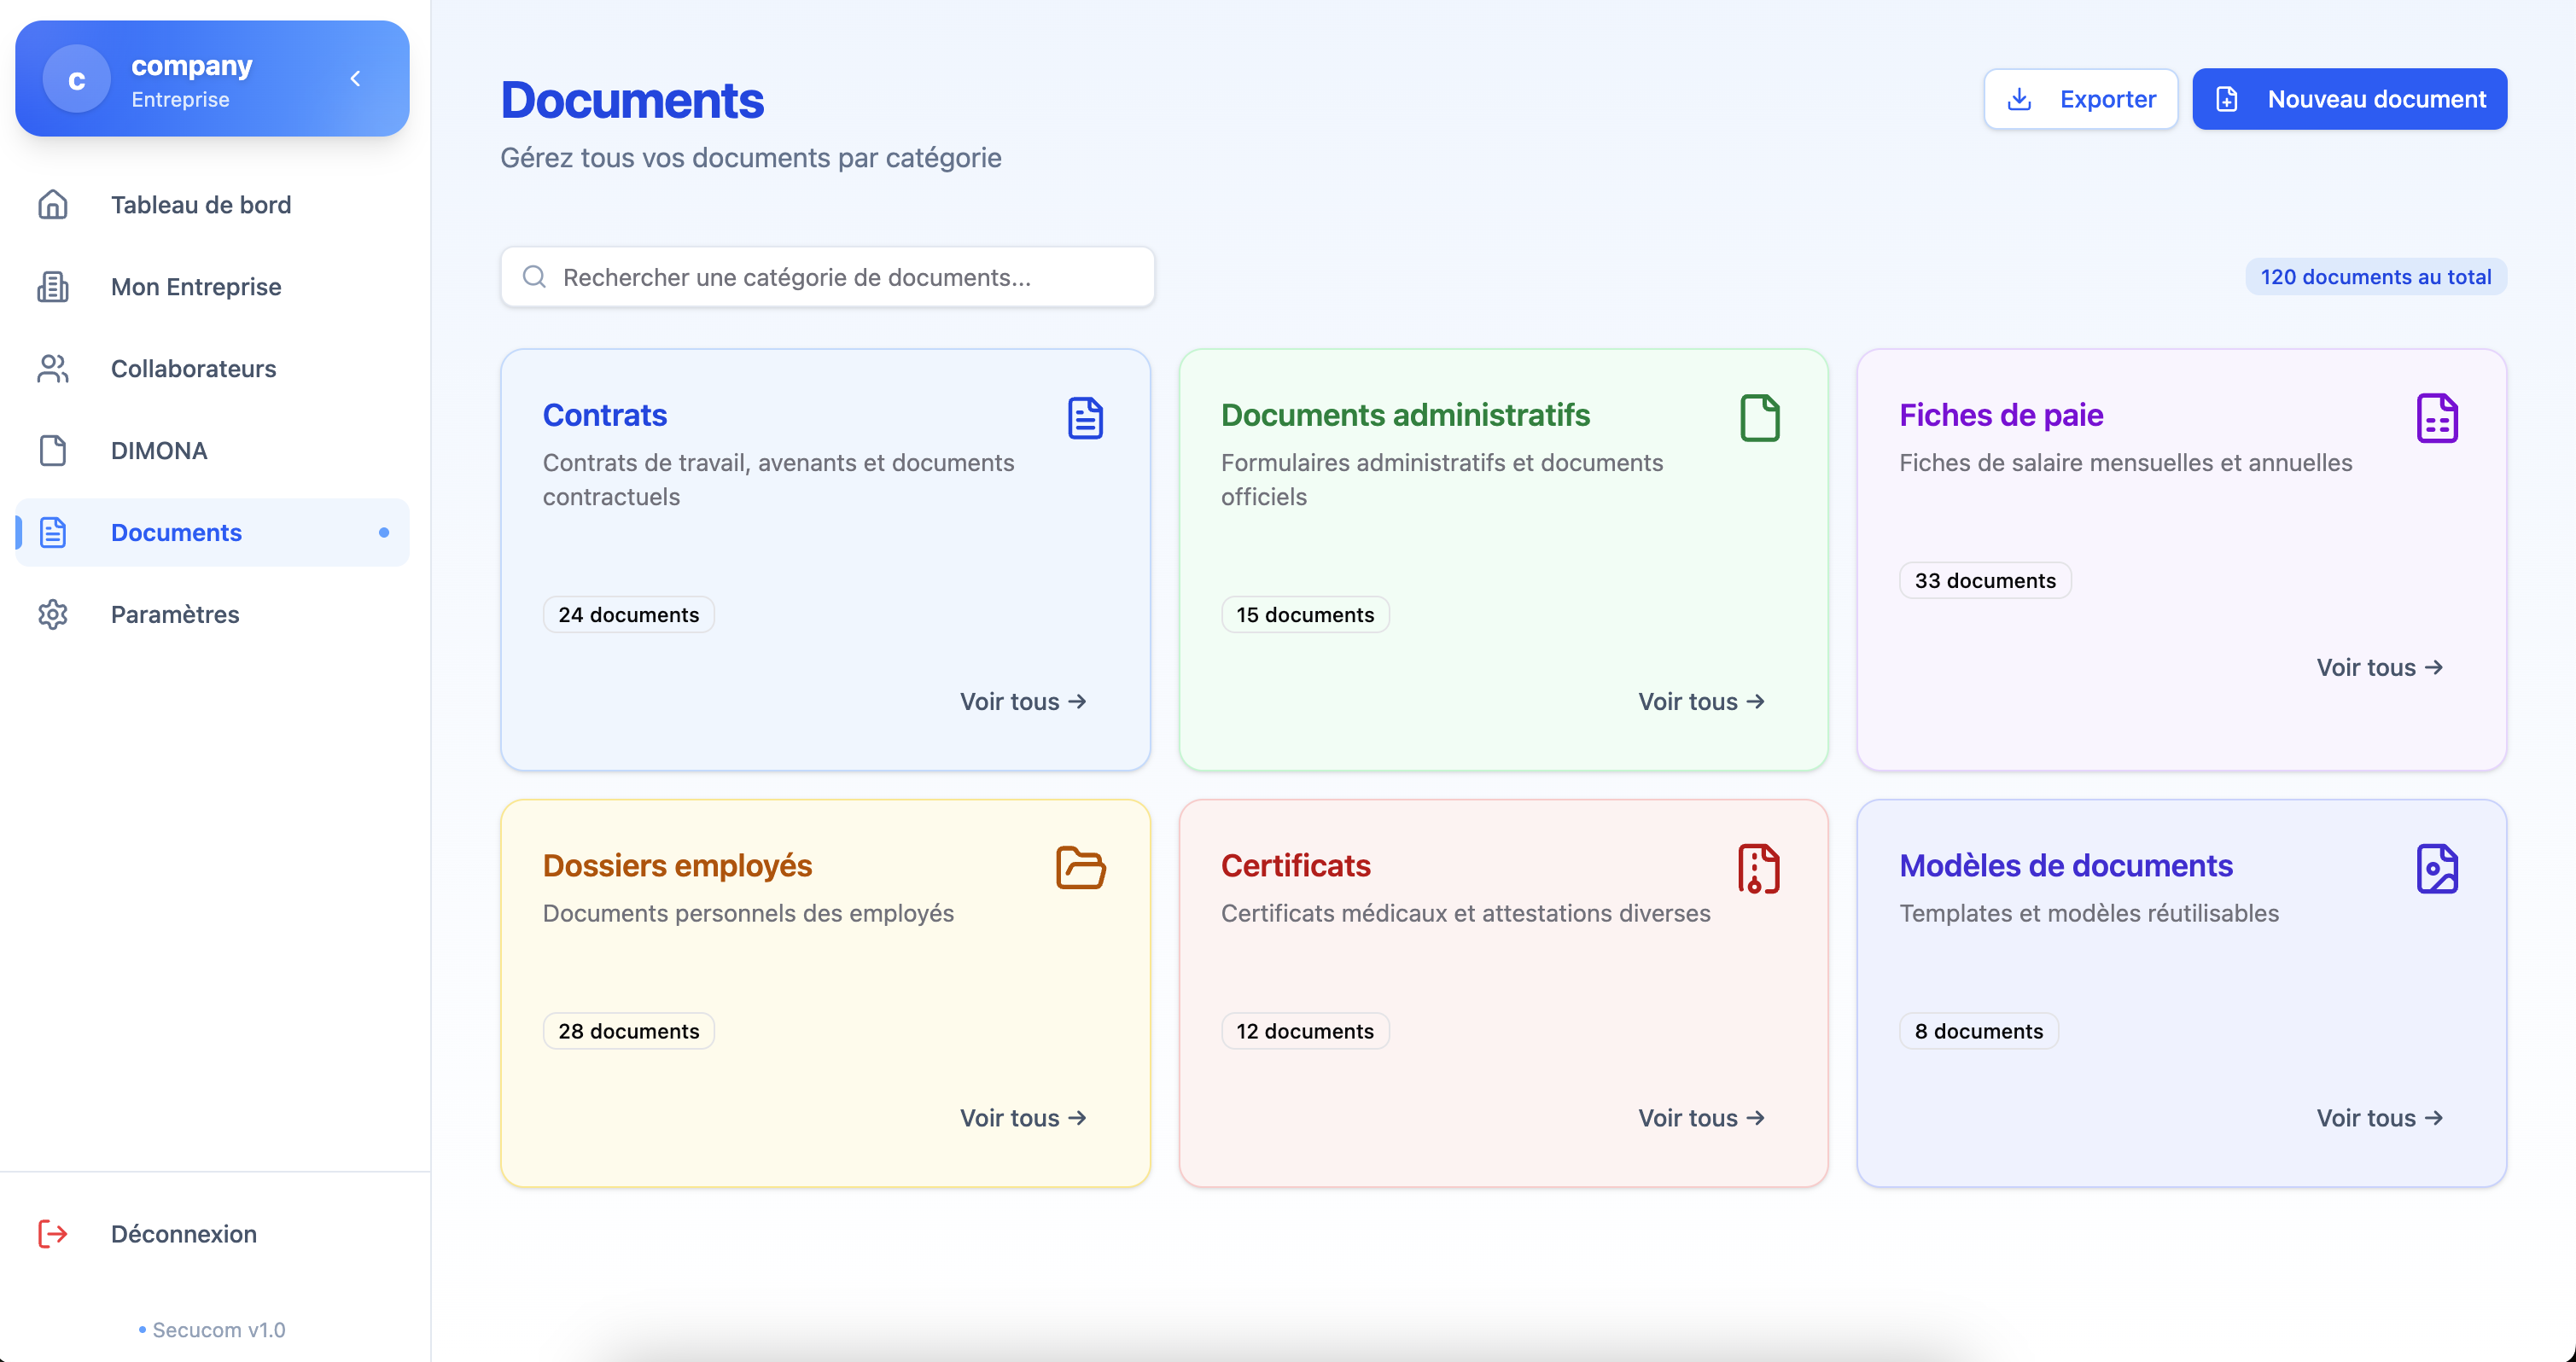
\includegraphics[width=0.9\textwidth]{SecuComPreviewDocs.png}
  \caption{Aperçu de l'interface de SecuCom}
  \label{fig:secucomPreview}
\end{figure}

\subsection{TypeScript}
\noindent Surcouche à JavaScript apportant un typage statique pour améliorer la détection précoce des erreurs et la maintenabilité du code.

\begin{note}
TypeScript réduit les erreurs à l'exécution, améliore la qualité du code et facilite la collaboration grâce à une meilleure documentation implicite.
\end{note}

\subsection{Tailwind CSS}
\noindent Framework CSS "utility-first" offrant flexibilité dans la conception tout en maintenant une cohérence visuelle.

\subsection{shadcnUI}
\noindent Collection de composants UI réutilisables construits avec Radix UI et stylisés avec Tailwind CSS, accélérant le développement tout en garantissant l'accessibilité et la modernité de l'interface.

\subsection{React Router DOM}
\noindent Bibliothèque gérant la navigation entre les différentes pages de l'application sans rechargement complet.

\section{Technologies back-end}

\subsection{Spring Boot}
\noindent Framework Java simplifiant le développement d'applications grâce à sa configuration automatique et ses conventions.

\subsection{Spring Security}
\noindent Module gérant l'authentification et l'autorisation, offrant une protection contre les attaques courantes et permettant une gestion fine des accès basée sur les rôles.

\subsection{Spring Data JPA}
\noindent Bibliothèque simplifiant l'accès aux données en réduisant le code boilerplate pour les opérations CRUD.

\subsection{Hibernate}
\noindent Implémentation de JPA facilitant la traduction entre les objets Java et les tables de la base de données.

\subsection{JSON Web Tokens (JWT)}
\noindent Mécanisme d'authentification sans état facilitant la scalabilité et éliminant le besoin de stocker des sessions côté serveur.

\begin{note}
JWT a été choisi pour son approche sans état, permettant une meilleure scalabilité et simplifiant la gestion des sessions utilisateurs.
\end{note}

\subsection{Base de données H2}
\noindent Base de données relationnelle légère choisie pour sa simplicité et sa capacité à gérer les relations entre entités.

\noindent Avantages dans le contexte de SecuCom :
\begin{itemize}[leftmargin=*,label=\textcolor{darkgray}{$\bullet$},itemsep=0.3em]
  \item Base embarquée sans installation séparée
  \item Compatibilité avec Spring Boot et Hibernate
  \item Fonctionnement en mémoire ou sur disque
  \item Console web intégrée pour le débogage
\end{itemize}

\begin{note}
H2 offre un bon compromis entre simplicité et fonctionnalités relationnelles. Une migration vers PostgreSQL ou MySQL serait possible pour un déploiement à grande échelle.
\end{note}

\section{Justification des choix technologiques}

\noindent Les technologies ont été sélectionnées selon quatre critères principaux :

\vspace{0.5cm}

\begin{figure}[h]
\centering
\begin{tabular}{|l|p{10cm}|}
\hline
\textbf{Critère} & \textbf{Application à SecuCom} \\
\hline
Adéquation fonctionnelle & 
\begin{itemize}[leftmargin=*,label=\textcolor{darkgray}{$\bullet$},itemsep=0.3em]
  \item Interface intuitive (ReactJS, Tailwind)
  \item Gestion de données complexes (Spring Data JPA, Hibernate)
  \item Sécurisation des accès (Spring Security, JWT)
\end{itemize} \\
\hline
Maturité et productivité & 
Écosystèmes Spring et ReactJS éprouvés avec communautés actives, offrant équilibre entre puissance et productivité \\
\hline
Maintenabilité et évolutivité & 
Architecture modulaire et séparation des responsabilités facilitant maintenance et évolution, TypeScript améliorant la robustesse du code \\
\hline
Pertinence professionnelle & 
Technologies valorisées sur le marché du travail, permettant de développer des compétences recherchées \\
\hline
\end{tabular}
\caption{Critères de sélection des technologies}
\end{figure}

\vspace{1cm}

\begin{tcolorbox}[
  title={\textbf{Cohérence technologique}},
  colback=blue!5!white,
  colframe=primarycolor,
  fonttitle=\bfseries,
  boxrule=0.5mm,
  arc=2mm,
  left=6mm,
  right=6mm,
  top=6mm,
  bottom=6mm
]
\noindent La stack technologique de SecuCom offre une cohérence entre frontend et backend, équilibrant :
\begin{itemize}[leftmargin=*,label=\textcolor{darkgray}{$\bullet$},itemsep=0.3em]
  \item Robustesse pour une application professionnelle
  \item Flexibilité pour l'adaptation aux besoins évolutifs
  \item Productivité pour un développement rapide
  \item Maintenabilité pour la pérennité de la solution
\end{itemize}

\noindent Cette approche permet à SecuCom d'évoluer pour répondre aux besoins de Sodabel et d'autres secrétariats sociaux.
\end{tcolorbox}
